% Options for packages loaded elsewhere
\PassOptionsToPackage{unicode}{hyperref}
\PassOptionsToPackage{hyphens}{url}
\PassOptionsToPackage{dvipsnames,svgnames,x11names}{xcolor}
\documentclass[
  11pt,
  a4paper,
]{article}
\usepackage{xcolor}
\usepackage[margin=24mm]{geometry}
\usepackage{amsmath,amssymb}
\setcounter{secnumdepth}{5}
\usepackage{iftex}
\ifPDFTeX
  \usepackage[T1]{fontenc}
  \usepackage[utf8]{inputenc}
  \usepackage{textcomp} % provide euro and other symbols
\else % if luatex or xetex
  \usepackage{unicode-math} % this also loads fontspec
  \defaultfontfeatures{Scale=MatchLowercase}
  \defaultfontfeatures[\rmfamily]{Ligatures=TeX,Scale=1}
\fi
\usepackage{lmodern}
\ifPDFTeX\else
  % xetex/luatex font selection
\fi
% Use upquote if available, for straight quotes in verbatim environments
\IfFileExists{upquote.sty}{\usepackage{upquote}}{}
\IfFileExists{microtype.sty}{% use microtype if available
  \usepackage[]{microtype}
  \UseMicrotypeSet[protrusion]{basicmath} % disable protrusion for tt fonts
}{}
\makeatletter
\@ifundefined{KOMAClassName}{% if non-KOMA class
  \IfFileExists{parskip.sty}{%
    \usepackage{parskip}
  }{% else
    \setlength{\parindent}{0pt}
    \setlength{\parskip}{6pt plus 2pt minus 1pt}}
}{% if KOMA class
  \KOMAoptions{parskip=half}}
\makeatother
\usepackage{longtable,booktabs,array}
\newcounter{none} % for unnumbered tables
\usepackage{calc} % for calculating minipage widths
% Correct order of tables after \paragraph or \subparagraph
\usepackage{etoolbox}
\makeatletter
\patchcmd\longtable{\par}{\if@noskipsec\mbox{}\fi\par}{}{}
\makeatother
% Allow footnotes in longtable head/foot
\IfFileExists{footnotehyper.sty}{\usepackage{footnotehyper}}{\usepackage{footnote}}
\makesavenoteenv{longtable}
\usepackage{graphicx}
\makeatletter
\newsavebox\pandoc@box
\newcommand*\pandocbounded[1]{% scales image to fit in text height/width
  \sbox\pandoc@box{#1}%
  \Gscale@div\@tempa{\textheight}{\dimexpr\ht\pandoc@box+\dp\pandoc@box\relax}%
  \Gscale@div\@tempb{\linewidth}{\wd\pandoc@box}%
  \ifdim\@tempb\p@<\@tempa\p@\let\@tempa\@tempb\fi% select the smaller of both
  \ifdim\@tempa\p@<\p@\scalebox{\@tempa}{\usebox\pandoc@box}%
  \else\usebox{\pandoc@box}%
  \fi%
}
% Set default figure placement to htbp
\def\fps@figure{htbp}
\makeatother
\setlength{\emergencystretch}{3em} % prevent overfull lines
\providecommand{\tightlist}{%
  \setlength{\itemsep}{0pt}\setlength{\parskip}{0pt}}
% Shared style; used by generated, standalone LaTeX sources.
\usepackage{xcolor}
\usepackage{xurl}
\usepackage{fvextra}
\usepackage{etoolbox}
\usepackage{fancyhdr}
\usepackage{titlesec}
\definecolor{researchblue}{HTML}{173B58}
\AtBeginDocument{\hypersetup{linkcolor=researchblue,urlcolor=researchblue}}
\pagestyle{fancy}
\fancyhf{}
\fancyhead[L]{\small\sffamily SVG PATCH LAB}
\fancyhead[R]{\small\sffamily CVPR 2027 research package}
\fancyfoot[L]{\small Working documents; results and proposals distinguished}
\fancyfoot[R]{\thepage}
\setlength{\headheight}{15pt}
\setlength{\emergencystretch}{3em}
\titleformat{\section}{\Large\bfseries\color{researchblue}}{\thesection}{0.7em}{}
\titleformat{\subsection}{\large\bfseries\color{researchblue}}{\thesubsection}{0.7em}{}
\DefineVerbatimEnvironment{verbatim}{Verbatim}{breaklines=true,breakanywhere=true,fontsize=\small}
\AtBeginEnvironment{longtable}{\small\setlength{\tabcolsep}{4pt}}
\let\originaltableofcontents\tableofcontents
\renewcommand{\tableofcontents}{\originaltableofcontents\clearpage}
\usepackage{bookmark}
\IfFileExists{xurl.sty}{\usepackage{xurl}}{} % add URL line breaks if available
\urlstyle{same}
\hypersetup{
  pdftitle={Auditing Numerical Claims in Editable Engineering SVGs},
  pdfauthor={SVG Patch Lab - Research Working Package},
  colorlinks=true,
  linkcolor={Maroon},
  filecolor={Maroon},
  citecolor={Blue},
  urlcolor={blue},
  pdfcreator={LaTeX via pandoc}}

\title{Auditing Numerical Claims in Editable Engineering SVGs}
\author{SVG Patch Lab - Research Working Package}
\date{14 September 2026 \textbar{} CVPR 2027 target}

\begin{document}
\maketitle

{
\setcounter{tocdepth}{2}
\tableofcontents
}
\textbf{Working manuscript for a prospective CVPR 2027 submission.} The
results below are implementation controls and an exploratory re-audit.
They do not yet establish a complete research contribution. Main
benchmark experiments, drafting assessment and author review remain
outstanding. This document is not formatted as a final conference
submission.

\section{Abstract}\label{abstract}

Scientific vector drawings can be syntactically valid and visually
plausible while making incorrect numerical claims. Editing introduces
further failure modes: changing an ancestor transform can alter a
contour without changing its path string, and editing a text label can
falsify a drawing while preserving every curve. We study the interface
between a numerical solution and its editable SVG representation. We
implement a sampled contour audit with ancestor transforms, arc-length
weighting, required-level coverage and explicit unsupported-reference
status, and examine a restricted editing policy that separates
presentation changes from physical changes requiring a new solve. On 160
manufactured controls, the geometric audit accepts 20 of 120 corrupted
drawings, all with wrong text labels; a rigid document-freeze baseline
accepts none. Re-auditing six historical generated drawings gives three
strict geometric passes, with the remaining cases exposing
corner-reference ambiguity, masked boundary coverage and an empty model
response. These findings motivate joint geometric and semantic checking,
but also show why numerical checks or constrained editing alone are
insufficient novelty claims. A small synthetic training pilot validates
the implementation pipeline; a perfect template-rule baseline limits
what its neural scores can demonstrate.

\section{Introduction}\label{introduction}

An engineering drawing is both an image and a collection of claims. A
curve labeled as an isotherm asserts that the temperature along the
curve equals a specified value. A stress legend asserts that its colors
refer to a particular derived quantity and unit. An edit that preserves
appearance can violate these assertions, while an edit that changes
appearance can preserve them exactly.

Recent systems already use language models to formulate and execute
simulations, generate scientific vector graphics, and modify editable
diagrams. The research problem is therefore not whether an LLM can call
a solver or output SVG. The question is whether the final editable
artifact remains consistent with the numerical solution it purports to
depict, particularly after a sequence of natural-language edits.

We distinguish three questions. First, does the numerical solution
adequately approximate the specified physical model? Second, does the
displayed geometry agree with that solution within a stated numerical
tolerance? Third, do the drawing's labels, units, legends and visibility
agree with the intended claims? A successful solver invocation addresses
neither of the latter two automatically. A low contour error does not
establish semantic or visual correctness.

The current work provides an implementation and diagnostic evidence for
this separation. The proposed submission must additionally establish
that a solver-linked representation improves useful editing under a
strong deterministic and prompting baseline, at comparable drafting
quality. Without that evidence, the contribution is a useful engineering
audit rather than a demonstrated new computer-vision method.

\section{Related work and
positioning}\label{related-work-and-positioning}

\textbf{Language-driven simulation.} MechAgents uses collaborating
language-model agents to write, execute and correct mechanics
simulations. Its examples include corrections to the plotted stress
quantity, making it directly relevant to the problem of
simulation-to-figure fidelity {[}1{]}. MCP-SIM maps natural-language
problems into simulation workflows through clarification, execution and
feedback {[}2{]}. We build on this workflow concept rather than claiming
the first LLM/solver integration. Reproduction remains necessary:
inspected MCP-SIM code lacks some imported utilities and
orchestration/dependency files, and MechAgents examples depend on older
software versions. These observations concern the available releases,
not the validity of private paper experiments.

\textbf{Scientific vector generation and editing.} SSVG-Bench and LOOP
evaluate structural properties of generated scientific graphics {[}3{]}.
AutoFigure-Edit provides editable scientific illustrations and an SVG
editing interface {[}4{]}. SciDiagramEdit studies instruction-driven
revisions to scientific vector sources and execution-trace-based skill
evolution {[}5{]}. SVGEditBench V2 evaluates general SVG editing
{[}6{]}. These works rule out broad claims to introduce structural
evaluation or instruction-based scientific SVG editing. A prospective
contribution should show benefits on numerical field claims and
sequential physical edits that their original benchmarks do not measure.

\textbf{Semantic constraints.} Penrose separates mathematical content
from visual styling and optimizes diagram layout under constraints
{[}7{]}. This motivates separating immutable physical meaning from
editable presentation. A numerical contour, however, also requires a
solution record, physical-coordinate mapping and explicit approximation
error. A useful baseline is a deterministic solver plot with frozen
geometry and templated labels: it may preserve claims perfectly while
offering limited layout flexibility.

\textbf{Learned simulation and preference training.} PINNs and
text-conditioned physics models are established alternatives for
approximating fields {[}8,9{]}. Their approximation and training costs
must be distinguished from the cost of drafting a figure. SciForma
studies scientific methodology diagrams with component, arrow and text
objectives {[}10{]}. Its diffusion renderer is adjacent to this task but
is not a native SVG/PDE baseline. We do not train a PINN simply to
supply a neural component when a conventional solver already provides
the required reference.

The literature review is targeted rather than exhaustive. We have not
established that no prior work implements the entire proposed
representation. The defensible claim must be narrowed after reproducing
the closest available systems.

\begin{figure}
\centering
\pandocbounded{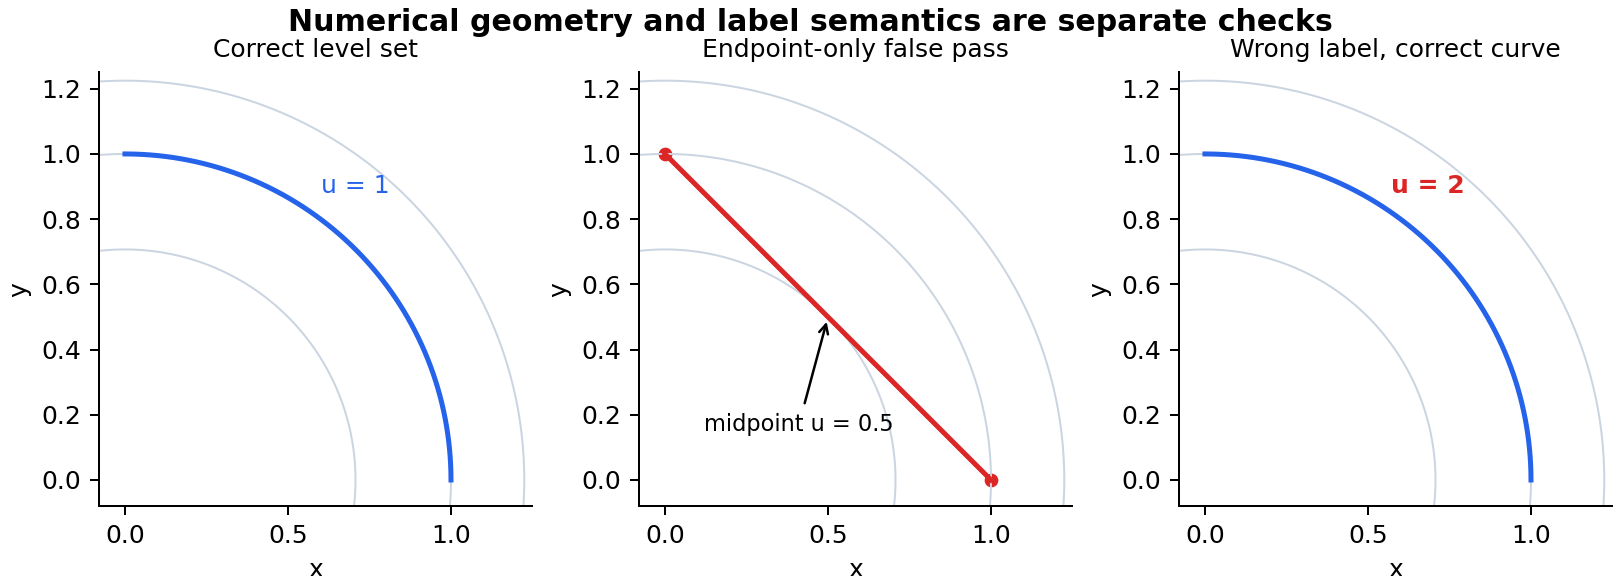
\includegraphics[keepaspectratio,alt={Geometric and semantic failure modes}]{../../paper/figures/failure_modes.png}}
\caption{Geometric and semantic failure modes}
\end{figure}

The follow-up FEM survey adds important direct precedents. FEABench
{[}17{]} evaluates end-to-end COMSOL operation; FEM-Bench {[}12{]} tests
FEM functions and generated tests; ALL-FEM {[}13{]} already fine-tunes
models on verified FEniCS programs and uses feedback-driven agents.
PDEAgent-Bench {[}14{]} evaluates numerical accuracy and efficiency
across PDE families and FEM libraries. OASiS {[}16{]} provides
multi-solver tooling and verification, while VFEAgent {[}15{]} addresses
image/text-to-FEA workflows. These works preclude novelty claims based
merely on solver calling, engineering-code fine-tuning, or adding
multimodal input. Our prospective contribution must concern the
correctness and usefulness of the final editable graphical artifact,
with direct comparisons and evidence still required.

\section{Problem formulation}\label{problem-formulation}

Let a physical problem be specified by domain geometry \(\Omega\),
governing equation P, boundary conditions B, material parameters
\(\theta\) and quantity q. A numerical solution record R stores these
inputs together with solver version, mesh or grid, units, convergence
diagnostics and an identifier. Let \(u_R\) be its scalar field and \(D\)
an SVG drawing associated with \(R\).

A contour claim consists of an SVG element identifier, a declared field
level c, a quantity and unit, and a mapping from SVG coordinates to
physical coordinates. The complete claim also includes its associated
label and legend entry. A physical input edit produces a new problem and
must invalidate the association with R until a new solution is
available. A presentation edit should preserve the claims while changing
only their visual arrangement or permitted style.

For a sampled contour with physical points \(x_i\) and arc-length
weights \(w_i\), define the mean normalized geometric error as

\[
E_{\mathrm{mean}} = 100\,\frac{\sum_i w_i\,|u_R(x_i)-c|}{\operatorname{range}_R\,\sum_i w_i}.
\]

We also report the maximum sampled error, required-level coverage,
invalid-reference samples and unsupported rendering features. The field
range is explicitly specified by the benchmark; it is not inferred
differently for each edited output. A strict pass requires every
required level, valid support for all checked samples, no flagged
unsupported condition, and maximum sampled error below the stated
tolerance.

This is a numerical audit, not a mathematical certificate. Finite
sampling cannot prove correctness between samples. Reference
interpolation has its own approximation error. Unsupported points must
not silently disappear from a pass/fail denominator.

\section{Implementation}\label{implementation}

\subsection{Geometric audit}\label{geometric-audit}

The previous local evaluator could reduce straight segments and arcs to
their endpoints. For \texttt{u(x,y)=x\^{}2+y\^{}2}, the chord from (1,0)
to (0,1) has endpoint value 1 at both ends but midpoint value 0.5. An
endpoint test can therefore report zero error for a visibly and
numerically incorrect level set.

The repaired evaluator parses SVG paths, including arcs and reflected
curve controls, and composes ancestor and local transforms. For Bezier
segments, a derivative-control-point bound determines a sampling
interval; arcs use a radius/angle bound and the affine operator norm.
Samples include segment endpoints and never introduce bridges between
disconnected subpaths. Chord-length quadrature approximates arc-length
weighting.

Bilinear interpolation retains out-of-domain or masked samples as
invalid coverage. A masked corner with exactly zero interpolation weight
is not treated as a contributing value. Missing levels, malformed
geometry and explicitly unsupported dynamic or rendering features
prevent a strict geometric pass. The implementation always reports that
a full drawing has not been verified.

\subsection{Restricted editing policy}\label{restricted-editing-policy}

The pilot executor owns the generated SVG and exposes a small action
schema: visible contour color, bounded stroke width, moving a bound
label within an annotation panel, routing a changed physical boundary
for recomputation, or rejecting a misleading request. The policy model
receives a compact DOM index and produces one JSON action. It does not
generate the numerical contour paths.

The executor rejects geometry, level and transform mutations through
this interface. Label text remains bound to the stored contour. A
recomputation action returns a pending solver request and never
certifies the old field as a new solution. This implementation supports
only its generated schema, not arbitrary user SVGs.

Crucially, the executor does not understand the instruction. A model can
choose a permitted action that does not fulfill the request. Thus we
evaluate exact action fulfillment separately from executor acceptance
and from geometry preservation. Arbitrary occlusion, label collision,
legend consistency and complete SVG rendering semantics remain outside
this pilot.

\section{Diagnostic experiments}\label{diagnostic-experiments}

\subsection{Manufactured corruption
controls}\label{manufactured-corruption-controls}

We generate 20 quarter-circle contour cases in the quadratic field
\texttt{u=x\^{}2+y\^{}2}. Each case has two honest variants (unchanged
and recolored) and six corruptions: replace an arc with its chord,
translate an ancestor, change the declared level, hide the contour,
remove it, or falsify its text label. All cases are simple
implementation controls with known construction; they are not samples of
natural model failures.

{\def\LTcaptype{none} % do not increment counter
\begin{longtable}[]{@{}lrr@{}}
\toprule\noalign{}
Checker & Honest accepted, n=40 & Corrupt accepted, n=120 \\
\midrule\noalign{}
\endhead
\bottomrule\noalign{}
\endlastfoot
Endpoint/local-coordinate control & 40/40 & 80/120 \\
Path-string hash protection & 40/40 & 80/120 \\
Repaired geometric audit & 40/40 & 20/120 \\
Rigid freeze except contour color & 40/40 & 0/120 \\
\end{longtable}
}

The numerical audit's remaining false accepts are all wrong-label cases.
This demonstrates the need for semantic checks; it does not demonstrate
superiority over the rigid baseline. The proposed method must retain
useful editing flexibility beyond the narrow recoloring task to justify
its additional complexity.

\begin{figure}
\centering
\pandocbounded{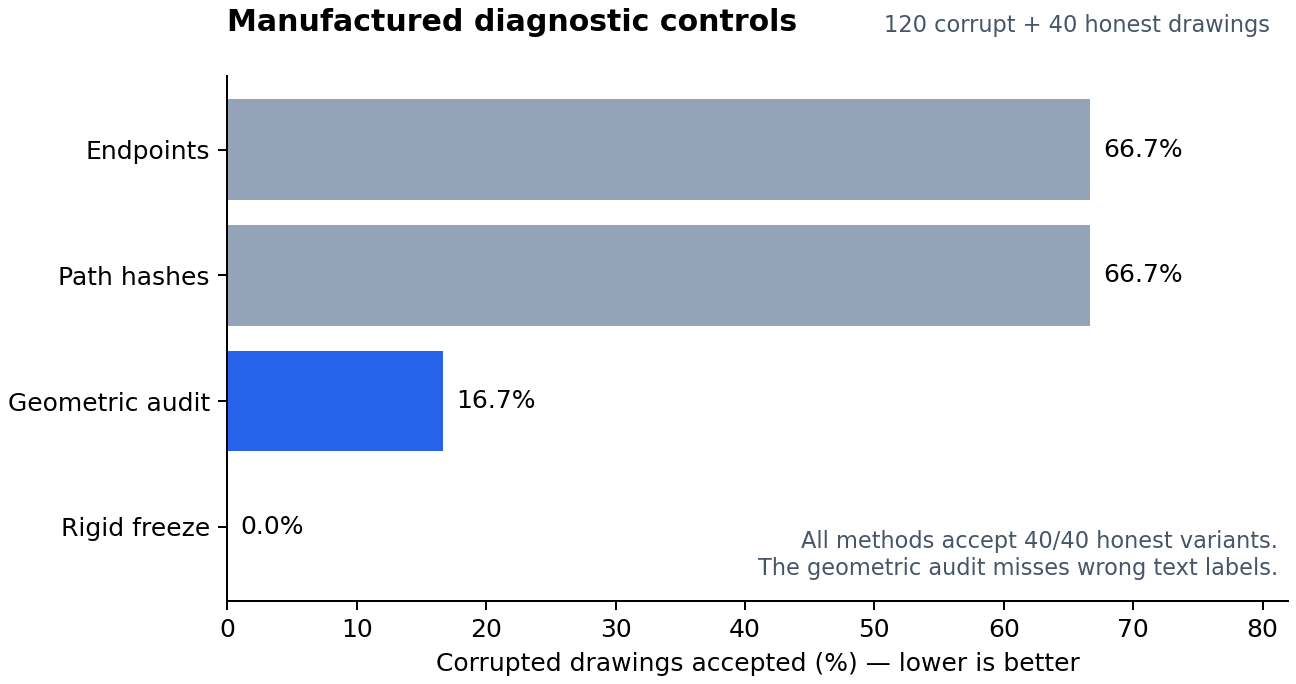
\includegraphics[keepaspectratio,alt={Manufactured corruption controls}]{../../paper/figures/corruption_controls.png}}
\caption{Manufactured corruption controls}
\end{figure}

\subsection{Exploratory historical
re-audit}\label{exploratory-historical-re-audit}

We re-score six pre-existing v3 generation attempts using a maximum
sampled error threshold of 0.5 percentage points of the specified field
range. The outputs and references were fixed before this repair. The
threshold and revised audit are exploratory, not a prospectively
preregistered evaluation.

{\def\LTcaptype{none} % do not increment counter
\begin{longtable}[]{@{}
  >{\raggedright\arraybackslash}p{(\linewidth - 4\tabcolsep) * \real{0.3000}}
  >{\raggedleft\arraybackslash}p{(\linewidth - 4\tabcolsep) * \real{0.4000}}
  >{\raggedright\arraybackslash}p{(\linewidth - 4\tabcolsep) * \real{0.3000}}@{}}
\toprule\noalign{}
\begin{minipage}[b]{\linewidth}\raggedright
Attempt
\end{minipage} & \begin{minipage}[b]{\linewidth}\raggedleft
Mean / maximum error, pp
\end{minipage} & \begin{minipage}[b]{\linewidth}\raggedright
Strict geometric outcome
\end{minipage} \\
\midrule\noalign{}
\endhead
\bottomrule\noalign{}
\endlastfoot
L-shaped Laplace & 0.3537 / 80.0000 & Does not pass; incompatible-corner
issue \\
Square torsion & 0.0701 / 0.3330 & Pass \\
Plate with square hole & 0.0693 / 0.2677 & Pass \\
Channel step streamlines & 0.0140 / 0.2459 & Pass \\
Square conductor in shell & 0.2167 / 0.3791 & Does not pass; 1,528
unsupported reference samples \\
Convective-edge plate & Not available & Empty response; counted as
attempted \\
\end{longtable}
}

The L-shaped case's largest errors occur at discontinuous/incompatible
corner boundary data. The shell's unsupported points occur on boundary
contours intersecting the raster reference mask, while its required
interior contours have valid support. These cases must not be
indiscriminately labeled incorrect model physics. A boundary protocol
and reference convergence study are needed. Full-domain results and any
prespecified exclusions should be reported together.

\subsection{Neural training pilot}\label{neural-training-pilot}

The pilot contains 60 training physical cases with six edits each, and
10 cases each for validation, test and held-out annuli. The rectangular
field is solved by finite differences and checked against the analytic
linear-temperature solution. The annular field uses the analytic radial
Laplace solution. All edit variants of a physical case remain in one
split.

We train attention-projection LoRA adapters on
Qwen2.5-Coder-1.5B-Instruct {[}11{]}, with rank 16, scale 32 and dropout
0.05. The A100 configuration uses FP16 frozen weights, microbatches of
four and three accumulation steps, with three fixed epochs and seeds 17,
29 and 41. The loss masks prompt tokens. Final checkpoints are fixed by
epoch count; held-out scores do not choose the model.

Evaluation retains every raw generation and counts every attempted
example. Strict JSON exact-action accuracy is reported alongside a
sensitivity score that removes only a single enclosing Markdown JSON
fence. Multiple objects, incomplete JSON and explanations are not
selectively parsed into a favorable action. This distinction was added
after inspecting formatting failures in the interrupted T4 diagnostic,
and is therefore a disclosed post-hoc diagnostic there and a specified
measure for the subsequent A100 runs.

All three A100 runs completed three epochs and 90 optimizer steps;
locally saved adapters, checkpoints and raw generations were verified.
Each final adapter obtains 60/60 strict exact actions on both evaluation
splits. The base obtains 0/60 under strict JSON parsing and 26/60 (test)
and 25/60 (annulus) after removing one enclosing JSON fence. The
deterministic template parser obtains 60/60 on both splits. Consequently
these results validate the training pipeline and do not establish a
benefit from learning. See \nolinkurl{../reports/TRAINING_RESULTS.md}
for configuration, recovery provenance and limitations.

\subsection{Direct API and FEM
recheck}\label{direct-api-and-fem-recheck}

Four new direct OpenAI Astra calls revisit the convective plate,
capacitor and bracket. Both Robin calls now return contours and finish
normally, including the 16,000-token condition that previously returned
nothing. One sample per condition does not estimate reliability or
isolate a budget effect. Direct evaluation in an independent P2 FEM
field gives mean/maximum errors of 0.00702/0.11074 °C for the
16,000-token condition and 0.01247/0.37385 °C for 32,000 tokens. The
final FEM mesh has 147,456 triangles; its difference from the preceding
mesh is below 0.008 °C at sampled contour points. Both drawings pass the
existing 0.5 °C sampled geometric threshold. This does not separately
certify boundary angles or all rendered semantics.

\begin{figure}
\centering
\pandocbounded{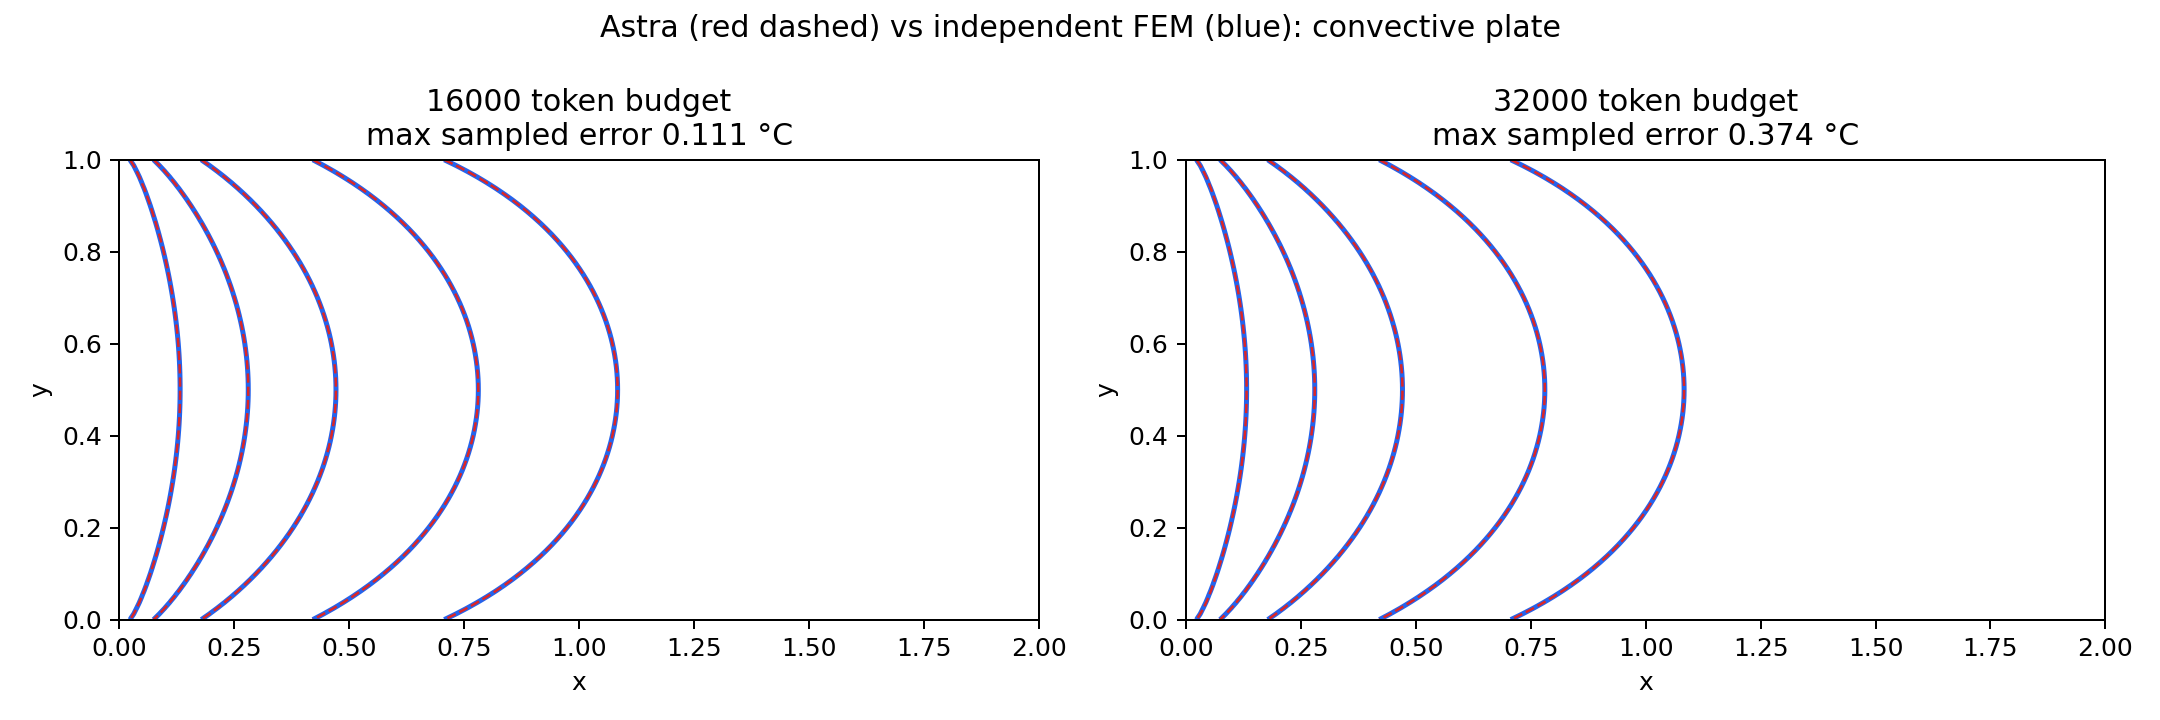
\includegraphics[keepaspectratio,alt={Astra and independent FEM}]{../../paper/figures/robin_fem_comparison.png}}
\caption{Astra and independent FEM}
\end{figure}

Inspection also corrects a qualitative claim in an older report: the
historical capacitor contains twelve open electric-field paths joining
conductors, not closed field loops, and labels the end contours
schematic. The bracket explicitly marks its stress map as illustrative
and identifies the need for geometry and restraint assumptions before
asserting a converged peak. These observations narrow the evidence: a
past completion failure is real, but these cases do not establish three
general classes of FEM incapability. Full evidence and protocol are in
\nolinkurl{../reports/ASTRA_FEM_FAILURE_RECHECK.md}.

\subsection{Reuse of an existing FEM
benchmark}\label{reuse-of-an-existing-fem-benchmark}

We begin extending FEM-Bench {[}12{]} by importing its unchanged
MIT-licensed axial-bar solver at a pinned commit. Both upstream
reference tests pass. Twelve generated cases and twelve load-edited
cases produce twenty-four actual FEM solves with analytic-displacement
and force-balance checks, numerical records and corresponding SVGs. This
replaces a routing-only demonstration with a real physical recomputation
in one elementary anchor. It is not a reproduction of FEM-Bench's full
evaluation, a new benchmark result, or evidence of a learned editing
advantage.

\section{Main study still required}\label{main-study-still-required}

The intended main study should compare direct SVG editing,
solver-informed unrestricted editing, protected geometry, joint
geometric/semantic protection, and deterministic solver plotting under
the same cases and instructions. Useful metrics include required-contour
coverage, field error, wrong quantity/unit rates, edit success,
disclosure and rejection correctness, render validity, drafting quality
and latency. Geometry-family and instruction-template holdouts should be
distinct evaluations.

At least three genuine numerical families should be included after
reference validation, such as Robin heat transfer, finite-domain
electrostatics and elasticity around a hole. Physical parameter edits
must trigger an actual solve. Multi-step sequences should test whether
prior protections survive later layout and semantic changes. Honest
counterfactuals are needed: a request to change a label to its
already-correct value should not be rejected merely because it contains
a relabeling verb.

Uncertainty should be computed over physical cases, not treated as if
six related edit variants were independent. Multiple training seeds,
compute accounting, mesh convergence, complete denominators and
qualitative failure inspection are necessary. Blinded drafting
assessment is needed to show the tradeoff between safety and useful
visual flexibility.

\section{Limitations and responsible
interpretation}\label{limitations-and-responsible-interpretation}

The present implementation does not establish full visible-figure
correctness or universal physical truth. Some SVG features are
explicitly unsupported; others, including arbitrary text semantics and
occlusion, are outside the geometric metric. Hashing a solution record
establishes identity, not that the solution is accurate or honestly
computed.

The manufactured controls are selected examples of vulnerabilities and
should not be used as an estimate of real-world prevalence. The
historical study is small and exploratory. The pilot task is templated,
language-only and solvable by a simple parser. There is no evidence here
that a neural editor outperforms a strong deterministic system in useful
drafting. These limitations determine the remaining experiments rather
than being hidden behind aggregate success rates.

\section{References}\label{references}

{[}1{]} Ni and Buehler. \emph{MechAgents: Large Language Model
Multi-Agent Collaborations Can Solve Mechanics Problems, Generate New
Data, and Integrate Knowledge.} \url{https://arxiv.org/abs/2311.08166} .
Author code: \url{https://github.com/lamm-mit/MechAgents} .

{[}2{]} Park, Moon and Ryu. \emph{MCP-SIM.} npj Artificial Intelligence,
2026. \url{https://www.nature.com/articles/s44387-025-00057-z} . Author
code: \url{https://github.com/KAIST-M4/MCP-SIM} .

{[}3{]} \emph{Towards the Generation of Structured Scientific Vector
Graphics with Large Language Models.} Inspected manuscript labeled under
review; acceptance unverified.
\url{https://openreview.net/pdf?id=aWypD2TAaC} .

{[}4{]} \emph{AutoFigure-Edit.} ACL System Demonstrations, 2026.
\url{https://aclanthology.org/2026.acl-demo.6/} .

{[}5{]} \emph{SciDiagramEdit.} Preprint, 2026.
\url{https://arxiv.org/abs/2607.15272} .

{[}6{]} \emph{SVGEditBench V2.} \url{https://arxiv.org/abs/2502.19453} .

{[}7{]} \emph{Penrose.} SIGGRAPH, 2020.
\url{https://penrose.ink/media/Penrose_SIGGRAPH2020.pdf} .

{[}8{]} Raissi et al.~\emph{Physics-informed neural networks.} Journal
of Computational Physics, 2019.
\url{https://www.sciencedirect.com/science/article/pii/S0021999118307125}
.

{[}9{]} \emph{Text2PDE.} \url{https://arxiv.org/abs/2410.01153} .

{[}10{]} \emph{SciForma.} Preprint, 2026.
\url{https://arxiv.org/abs/2607.18091} .

{[}11{]} Qwen. \emph{Qwen2.5-Coder-1.5B-Instruct.}
\url{https://huggingface.co/Qwen/Qwen2.5-Coder-1.5B-Instruct} .

Bibliographic entries are working source pointers. Verify complete
author lists, titles, publication status and BibTeX metadata before
submission.

{[}12{]} Mohammadzadeh, Hamdi, Shor and Lejeune. \emph{FEM-Bench: A
Structured Scientific Reasoning Benchmark for Evaluating Code-Generating
LLMs.} \url{https://arxiv.org/abs/2512.20732} . Code:
\url{https://github.com/elejeune11/FEM-bench} .

{[}13{]} Deotale et al.~\emph{ALL-FEM: Agentic Large Language Models
fine-tuned for finite element methods.} Computer Methods in Applied
Mechanics and Engineering 457:118985, 2026.
\url{https://doi.org/10.1016/j.cma.2026.118985} . Author project:
\url{https://fenics-llm.github.io/} .

{[}14{]} \emph{PDEAgent-Bench: A Multi-Metric, Multi-Library Benchmark
for PDE Solver Generation.} 2026. \url{https://arxiv.org/abs/2605.09636}
.

{[}15{]} Zhang et al.~\emph{VFEAgent: A Multimodal Agent Framework for
End-to-End Automated Finite Element Analysis.} Preprint, 2026.
\url{https://arxiv.org/abs/2605.28978} .

{[}16{]} Hermann, Shojaei, Scheider and Cyron. \emph{OASiS: an
open-source multi-physics and multi-code framework for verified computer
simulations.} Software, 2026.
\url{https://github.com/Hereon-InstituteMS/OASiS} .

{[}17{]} Mudur et al.~\emph{FEABench: Evaluating Language Models on
Multiphysics Reasoning Ability.} \url{https://arxiv.org/abs/2504.06260}
.

\end{document}
